\documentclass{article}
\title{CSC301 HW4}
\author{Alex Zhang}
\date{Feb 2023}


\usepackage{graphicx}
\graphicspath{ {./images/} }
\textwidth=16.00cm 
\textheight=22.00cm 
\topmargin=0.00cm
\oddsidemargin=0.00cm 
\evensidemargin=0.00cm 
\headheight=0cm 
\headsep=0.5cm
\textheight=610pt

\usepackage{amsthm,amssymb}
\usepackage{amsmath}

\newcommand{\bmat}[1]{\begin{bmatrix} #1 \end{bmatrix}}
\newcommand{\mat}[1]{\mathbf{#1}}
\newcommand{\mb}[1]{\mathbb{#1}}

\let\ds\displaystyle


\begin{document}
\maketitle
\section*{Question 1}
\paragraph{Proof:} $\mat{B} = \mat{A}\mat{A} = \mat{A}^2$

If there exists a path of length two between vertex $u$ and $w$, then $\exists $ $i$ which 
in adjacency matrix $\mat{A}$, both $\mat{a}_{ui}$ and $\mat{a}_{iw}$ exists.
In order to ensure both $\mat{a}_{ui}$ and $\mat{a}_{iw}$ exists, their product $\mat{a}_{ui} \cdot \mat{a}_{iw}$
has to be 1.

Since $\mat{B}$ is counting the number of two-paths in the given graph. With given vertex $u$, and vertex $w$, $\mat{B}_{uw}$
is just the sum of all exist two-paths. In mathematical expression $$\mat{B}_{uw} = \sum^{n}_{i=0}\mat{a}_{ui}\cdot \mat{a}_{iw}$$
Also by the definition of matrix multiplication, 
$$\mat{A}\mat{A}_{uw} = \sum^{n}_{i=0}\mat{a}_{ui}\cdot \mat{a}_{iw}$$
for all vertex $u$ and $w$. This implies that,
$\mat{B} = \mat{A}\mat{A} = \mat{A}^2$.$\blacksquare$

\section*{Question 2}
In matrixMult.java file, different methods are created. The randMat method is used to random generate a n by n dimention
matrix and put it into text file. The matTransform method is used to transform tex file matrix into array representation.
The multiplication method is matrix multiplication using strassens's method. The print method is just printing matrix in 2-D order.
The user can change the value of n in order to perfrom matrix multiplication on different dimention. There are also two unit test included.
\\
I have added more descriptions of my code through comments in JAVA file.



\section*{Question 3}
\subsection*{(a)}
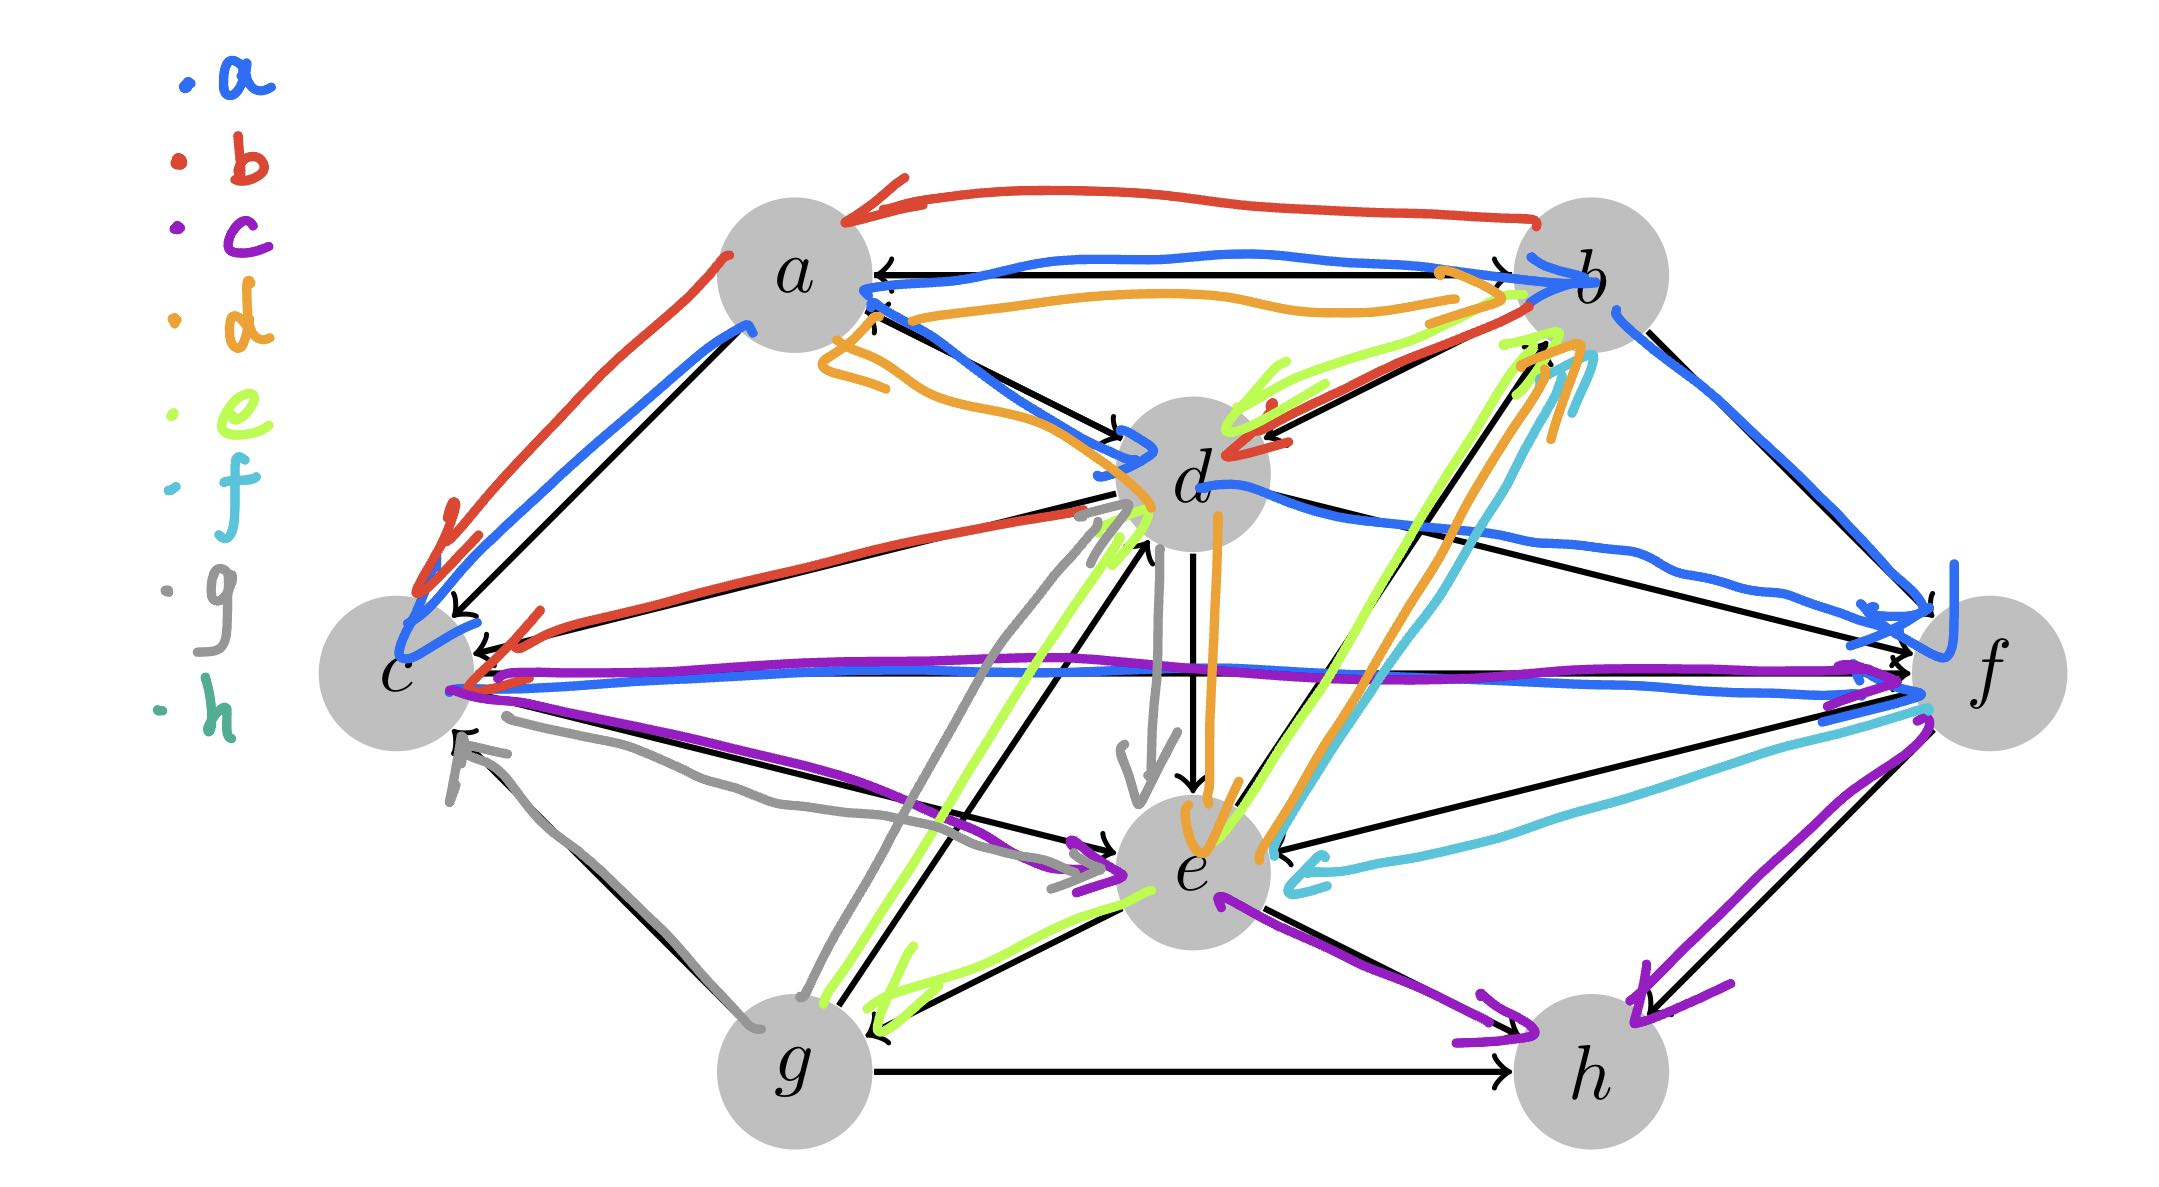
\includegraphics[scale = 0.25]{graph.jpg}

\begin{enumerate}
    \item For $a$, the best recommander should be $f$ since the number of two-paths is 3.
    \item For $b$, the best recommander should be $c$ since it has the most two-paths 2.
    \item For $c$, the best recommander should be $h$ since it has 2 two-paths which is the most
    \item For $d$, the best recommander should be $h$. $b$ and $e$ also have the same number of two-paths, but they have already connected to $d$ which we should recommand $h$.
    \item For $e$, the best recommander should be $d$ since it has the most number of two-paths of 2.
    \item For $f$, the best recommander should be $b$. Because $b$, $e$, and $f$ all have same two-paths, by alphabetical order, we should choose $b$.
    \item For $g$, the best recommander should be $e$ since $e$ and $f$ have the same two-paths and by alphabetical order we choose $e$.
    \item For $h$, the best recommander should be $a$. Because for any letter the number of two-paths is 0 which lead us to choose $a$.
\end{enumerate}

\subsection*{(b)}
Based on the graph, we can create an adjacency matrix 
$$\mat{A} = \begin{bmatrix}
    \ & a & b & c & d & e & f & g & h \\
    a & 0 & 1 & 1 & 1 & 0 & 0 & 0 & 0 \\
    b & 1 & 0 & 0 & 1 & 0 & 1 & 0 & 0 \\
    c & 0 & 0 & 0 & 0 & 1 & 1 & 0 & 0 \\
    d & 0 & 0 & 1 & 0 & 1 & 1 & 0 & 0 \\
    e & 0 & 1 & 0 & 0 & 0 & 0 & 1 & 1 \\
    f & 0 & 0 & 0 & 0 & 1 & 0 & 0 & 1 \\
    g & 0 & 0 & 1 & 1 & 0 & 0 & 0 & 1 \\
    h & 0 & 0 & 0 & 0 & 0 & 0 & 0 & 0 
\end{bmatrix}
$$
\subsection*{(c)}
After doing the computation in Task(2), I got the following matrix $\mat{B}$,
$$\begin{bmatrix}
1& 0 &1& 1& 2& 3& 0& 0\\
0& 1& 2& 1& 2& 1& 0& 1\\
0& 1& 0& 0& 1& 0& 1& 2\\
0& 1& 0& 0& 2& 1& 1& 2\\
1& 0& 1& 2& 0& 1& 0& 1\\
0& 1& 0& 0& 0& 0& 1& 1\\
0& 0& 1& 0& 2& 2& 0& 0\\
0& 0& 0& 0& 0& 0& 0& 0
\end{bmatrix}$$
\subsection*{(d)}
Based on the $\mat{B}$ we have calculated, we can just look
at the entries to determine best recommander.
\begin{enumerate}
    \item For $a$, recommander should be $f$.
    \item For $b$, recommander should be $c$.
    \item For $c$, recommander should be $h$.
    \item For $d$, recommander should be $h$.
    \item For $e$, recommander should be $d$.
    \item For $f$, recommander should be $b$.
    \item For $g$, recommander should be $e$.
    \item For $h$, recommander should be $a$.
\end{enumerate}
I think based on the matrix $\mat{B}$ and the ties rule, the recommendation from $\mat{B}$
matches the recommendation from Task(3a).




\end{document}